
%% bare_conf_compsoc.tex
%% V1.4b
%% 2015/08/26
%% by Michael Shell
%% See:
%% http://www.michaelshell.org/
%% for current contact information.
%%
%% This is a skeleton file demonstrating the use of IEEEtran.cls
%% (requires IEEEtran.cls version 1.8b or later) with an IEEE Computer
%% Society conference paper.
%%
%% Support sites:
%% http://www.michaelshell.org/tex/ieeetran/
%% http://www.ctan.org/pkg/ieeetran
%% and
%% http://www.ieee.org/

%%*************************************************************************
%% Legal Notice:
%% This code is offered as-is without any warranty either expressed or
%% implied; without even the implied warranty of MERCHANTABILITY or
%% FITNESS FOR A PARTICULAR PURPOSE! 
%% User assumes all risk.
%% In no event shall the IEEE or any contributor to this code be liable for
%% any damages or losses, including, but not limited to, incidental,
%% consequential, or any other damages, resulting from the use or misuse
%% of any information contained here.
%%
%% All comments are the opinions of their respective authors and are not
%% necessarily endorsed by the IEEE.
%%
%% This work is distributed under the LaTeX Project Public License (LPPL)
%% ( http://www.latex-project.org/ ) version 1.3, and may be freely used,
%% distributed and modified. A copy of the LPPL, version 1.3, is included
%% in the base LaTeX documentation of all distributions of LaTeX released
%% 2003/12/01 or later.
%% Retain all contribution notices and credits.
%% ** Modified files should be clearly indicated as such, including  **
%% ** renaming them and changing author support contact information. **
%%*************************************************************************


% *** Authors should verify (and, if needed, correct) their LaTeX system  ***
% *** with the testflow diagnostic prior to trusting their LaTeX platform ***
% *** with production work. The IEEE's font choices and paper sizes can   ***
% *** trigger bugs that do not appear when using other class files.       ***                          ***
% The testflow support page is at:
% http://www.michaelshell.org/tex/testflow/



\documentclass[conference,compsoc]{IEEEtran}
% Some/most Computer Society conferences require the compsoc mode option,
% but others may want the standard conference format.
%
% If IEEEtran.cls has not been installed into the LaTeX system files,
% manually specify the path to it like:
% \documentclass[conference,compsoc]{../sty/IEEEtran}





% Some very useful LaTeX packages include:
% (uncomment the ones you want to load)


% *** MISC UTILITY PACKAGES ***
%
%\usepackage{ifpdf}
% Heiko Oberdiek's ifpdf.sty is very useful if you need conditional
% compilation based on whether the output is pdf or dvi.
% usage:
% \ifpdf
%   % pdf code
% \else
%   % dvi code
% \fi
% The latest version of ifpdf.sty can be obtained from:
% http://www.ctan.org/pkg/ifpdf
% Also, note that IEEEtran.cls V1.7 and later provides a builtin
% \ifCLASSINFOpdf conditional that works the same way.
% When switching from latex to pdflatex and vice-versa, the compiler may
% have to be run twice to clear warning/error messages.






% *** CITATION PACKAGES ***
%
\ifCLASSOPTIONcompsoc
  % IEEE Computer Society needs nocompress option
  % requires cite.sty v4.0 or later (November 2003)
  \usepackage[nocompress]{cite}
\else
  % normal IEEE
  \usepackage{cite}
\fi

\usepackage{caption}
\usepackage{graphicx, subfigure}
\usepackage{algorithm}
\usepackage{algorithmic}
\usepackage{multirow}
\usepackage{amsmath,amssymb,amsfonts}
\renewcommand{\algorithmicrequire}{ \textbf{Input:}} %Use Input in the format of Algorithm
\renewcommand{\algorithmicensure}{ \textbf{Output:}} %UseOutput in the format of Algorithm


\renewcommand\thesection{\arabic{section}} 
\renewcommand\thesubsection{\thesection.\Alph{subsection}} 
% cite.sty was written by Donald Arseneau
% V1.6 and later of IEEEtran pre-defines the format of the cite.sty package
% \cite{} output to follow that of the IEEE. Loading the cite package will
% result in citation numbers being automatically sorted and properly
% "compressed/ranged". e.g., [1], [9], [2], [7], [5], [6] without using
% cite.sty will become [1], [2], [5]--[7], [9] using cite.sty. cite.sty's
% \cite will automatically add leading space, if needed. Use cite.sty's
% noadjust option (cite.sty V3.8 and later) if you want to turn this off
% such as if a citation ever needs to be enclosed in parenthesis.
% cite.sty is already installed on most LaTeX systems. Be sure and use
% version 5.0 (2009-03-20) and later if using hyperref.sty.
% The latest version can be obtained at:
% http://www.ctan.org/pkg/cite
% The documentation is contained in the cite.sty file itself.
%
% Note that some packages require special options to format as the Computer
% Society requires. In particular, Computer Society  papers do not use
% compressed citation ranges as is done in typical IEEE papers
% (e.g., [1]-[4]). Instead, they list every citation separately in order
% (e.g., [1], [2], [3], [4]). To get the latter we need to load the cite
% package with the nocompress option which is supported by cite.sty v4.0
% and later.





% *** GRAPHICS RELATED PACKAGES ***
%
\ifCLASSINFOpdf
  % \usepackage[pdftex]{graphicx}
  % declare the path(s) where your graphic files are
  % \graphicspath{{../pdf/}{../jpeg/}}
  % and their extensions so you won't have to specify these with
  % every instance of \includegraphics
  % \DeclareGraphicsExtensions{.pdf,.jpeg,.png}
\else
  % or other class option (dvipsone, dvipdf, if not using dvips). graphicx
  % will default to the driver specified in the system graphics.cfg if no
  % driver is specified.
  % \usepackage[dvips]{graphicx}
  % declare the path(s) where your graphic files are
  % \graphicspath{{../eps/}}
  % and their extensions so you won't have to specify these with
  % every instance of \includegraphics
  % \DeclareGraphicsExtensions{.eps}
\fi
% graphicx was written by David Carlisle and Sebastian Rahtz. It is
% required if you want graphics, photos, etc. graphicx.sty is already
% installed on most LaTeX systems. The latest version and documentation
% can be obtained at: 
% http://www.ctan.org/pkg/graphicx
% Another good source of documentation is "Using Imported Graphics in
% LaTeX2e" by Keith Reckdahl which can be found at:
% http://www.ctan.org/pkg/epslatex
%
% latex, and pdflatex in dvi mode, support graphics in encapsulated
% postscript (.eps) format. pdflatex in pdf mode supports graphics
% in .pdf, .jpeg, .png and .mps (metapost) formats. Users should ensure
% that all non-photo figures use a vector format (.eps, .pdf, .mps) and
% not a bitmapped formats (.jpeg, .png). The IEEE frowns on bitmapped formats
% which can result in "jaggedy"/blurry rendering of lines and letters as
% well as large increases in file sizes.
%
% You can find documentation about the pdfTeX application at:
% http://www.tug.org/applications/pdftex





% *** MATH PACKAGES ***
%
%\usepackage{amsmath}
% A popular package from the American Mathematical Society that provides
% many useful and powerful commands for dealing with mathematics.
%
% Note that the amsmath package sets \interdisplaylinepenalty to 10000
% thus preventing page breaks from occurring within multiline equations. Use:
%\interdisplaylinepenalty=2500
% after loading amsmath to restore such page breaks as IEEEtran.cls normally
% does. amsmath.sty is already installed on most LaTeX systems. The latest
% version and documentation can be obtained at:
% http://www.ctan.org/pkg/amsmath





% *** SPECIALIZED LIST PACKAGES ***
%
%\usepackage{algorithmic}
% algorithmic.sty was written by Peter Williams and Rogerio Brito.
% This package provides an algorithmic environment fo describing algorithms.
% You can use the algorithmic environment in-text or within a figure
% environment to provide for a floating algorithm. Do NOT use the algorithm
% floating environment provided by algorithm.sty (by the same authors) or
% algorithm2e.sty (by Christophe Fiorio) as the IEEE does not use dedicated
% algorithm float types and packages that provide these will not provide
% correct IEEE style captions. The latest version and documentation of
% algorithmic.sty can be obtained at:
% http://www.ctan.org/pkg/algorithms
% Also of interest may be the (relatively newer and more customizable)
% algorithmicx.sty package by Szasz Janos:
% http://www.ctan.org/pkg/algorithmicx




% *** ALIGNMENT PACKAGES ***
%
%\usepackage{array}
% Frank Mittelbach's and David Carlisle's array.sty patches and improves
% the standard LaTeX2e array and tabular environments to provide better
% appearance and additional user controls. As the default LaTeX2e table
% generation code is lacking to the point of almost being broken with
% respect to the quality of the end results, all users are strongly
% advised to use an enhanced (at the very least that provided by array.sty)
% set of table tools. array.sty is already installed on most systems. The
% latest version and documentation can be obtained at:
% http://www.ctan.org/pkg/array


% IEEEtran contains the IEEEeqnarray family of commands that can be used to
% generate multiline equations as well as matrices, tables, etc., of high
% quality.




% *** SUBFIGURE PACKAGES ***
%\ifCLASSOPTIONcompsoc
%  \usepackage[caption=false,font=footnotesize,labelfont=sf,textfont=sf]{subfig}
%\else
%  \usepackage[caption=false,font=footnotesize]{subfig}
%\fi
% subfig.sty, written by Steven Douglas Cochran, is the modern replacement
% for subfigure.sty, the latter of which is no longer maintained and is
% incompatible with some LaTeX packages including fixltx2e. However,
% subfig.sty requires and automatically loads Axel Sommerfeldt's caption.sty
% which will override IEEEtran.cls' handling of captions and this will result
% in non-IEEE style figure/table captions. To prevent this problem, be sure
% and invoke subfig.sty's "caption=false" package option (available since
% subfig.sty version 1.3, 2005/06/28) as this is will preserve IEEEtran.cls
% handling of captions.
% Note that the Computer Society format requires a sans serif font rather
% than the serif font used in traditional IEEE formatting and thus the need
% to invoke different subfig.sty package options depending on whether
% compsoc mode has been enabled.
%
% The latest version and documentation of subfig.sty can be obtained at:
% http://www.ctan.org/pkg/subfig




% *** FLOAT PACKAGES ***
%
%\usepackage{fixltx2e}
% fixltx2e, the successor to the earlier fix2col.sty, was written by
% Frank Mittelbach and David Carlisle. This package corrects a few problems
% in the LaTeX2e kernel, the most notable of which is that in current
% LaTeX2e releases, the ordering of single and double column floats is not
% guaranteed to be preserved. Thus, an unpatched LaTeX2e can allow a
% single column figure to be placed prior to an earlier double column
% figure.
% Be aware that LaTeX2e kernels dated 2015 and later have fixltx2e.sty's
% corrections already built into the system in which case a warning will
% be issued if an attempt is made to load fixltx2e.sty as it is no longer
% needed.
% The latest version and documentation can be found at:
% http://www.ctan.org/pkg/fixltx2e


%\usepackage{stfloats}
% stfloats.sty was written by Sigitas Tolusis. This package gives LaTeX2e
% the ability to do double column floats at the bottom of the page as well
% as the top. (e.g., "\begin{figure*}[!b]" is not normally possible in
% LaTeX2e). It also provides a command:
%\fnbelowfloat
% to enable the placement of footnotes below bottom floats (the standard
% LaTeX2e kernel puts them above bottom floats). This is an invasive package
% which rewrites many portions of the LaTeX2e float routines. It may not work
% with other packages that modify the LaTeX2e float routines. The latest
% version and documentation can be obtained at:
% http://www.ctan.org/pkg/stfloats
% Do not use the stfloats baselinefloat ability as the IEEE does not allow
% \baselineskip to stretch. Authors submitting work to the IEEE should note
% that the IEEE rarely uses double column equations and that authors should try
% to avoid such use. Do not be tempted to use the cuted.sty or midfloat.sty
% packages (also by Sigitas Tolusis) as the IEEE does not format its papers in
% such ways.
% Do not attempt to use stfloats with fixltx2e as they are incompatible.
% Instead, use Morten Hogholm'a dblfloatfix which combines the features
% of both fixltx2e and stfloats:
%
% \usepackage{dblfloatfix}
% The latest version can be found at:
% http://www.ctan.org/pkg/dblfloatfix




% *** PDF, URL AND HYPERLINK PACKAGES ***
%
%\usepackage{url}
% url.sty was written by Donald Arseneau. It provides better support for
% handling and breaking URLs. url.sty is already installed on most LaTeX
% systems. The latest version and documentation can be obtained at:
% http://www.ctan.org/pkg/url
% Basically, \url{my_url_here}.




% *** Do not adjust lengths that control margins, column widths, etc. ***
% *** Do not use packages that alter fonts (such as pslatex).         ***
% There should be no need to do such things with IEEEtran.cls V1.6 and later.
% (Unless specifically asked to do so by the journal or conference you plan
% to submit to, of course. )


% correct bad hyphenation here
\hyphenation{op-tical net-works semi-conduc-tor}



\begin{document}
%
% paper title
% Titles are generally capitalized except for words such as a, an, and, as,
% at, but, by, for, in, nor, of, on, or, the, to and up, which are usually
% not capitalized unless they are the first or last word of the title.
% Linebreaks \\ can be used within to get better formatting as desired.
% Do not put math or special symbols in the title.
\title{AAA: High Agile Adaptive Flow-Awareness \\ Network for SDN}


% author names and affiliations
% use a multiple column layout for up to three different
% affiliations
\author{He Cai$^{1}$, Jun Deng$^{1}$, Xiaofei Wang$^{1}$
\\
${^1}$Tianjin Key Laboratory of Advanced Networking, %School of Computer Science and Technology,\\
Tianjin University, Tianjin, China.
%\begin{small}
%*Prof. Keqiu Li is the corresponding author.
%\end{small}
}


% conference papers do not typically use \thanks and this command
% is locked out in conference mode. If really needed, such as for
% the acknowledgment of grants, issue a \IEEEoverridecommandlockouts
% after \documentclass

% for over three affiliations, or if they all won't fit within the width
% of the page (and note that there is less available width in this regard for
% compsoc conferences compared to traditional conferences), use this
% alternative format:
% 
%\author{\IEEEauthorblockN{Michael Shell\IEEEauthorrefmark{1},
%Homer Simpson\IEEEauthorrefmark{2},
%James Kirk\IEEEauthorrefmark{3}, 
%Montgomery Scott\IEEEauthorrefmark{3} and
%Eldon Tyrell\IEEEauthorrefmark{4}}
%\IEEEauthorblockA{\IEEEauthorrefmark{1}School of Electrical and Computer Engineering\\
%Georgia Institute of Technology,
%Atlanta, Georgia 30332--0250\\ Email: see http://www.michaelshell.org/contact.html}
%\IEEEauthorblockA{\IEEEauthorrefmark{2}Twentieth Century Fox, Springfield, USA\\
%Email: homer@thesimpsons.com}
%\IEEEauthorblockA{\IEEEauthorrefmark{3}Starfleet Academy, San Francisco, California 96678-2391\\
%Telephone: (800) 555--1212, Fax: (888) 555--1212}
%\IEEEauthorblockA{\IEEEauthorrefmark{4}Tyrell Inc., 123 Replicant Street, Los Angeles, California 90210--4321}}




% use for special paper notices
%\IEEEspecialpapernotice{(Invited Paper)}




% make the title area
\maketitle

% As a general rule, do not put math, special symbols or citations
% in the abstract
\begin{abstract}
The abstract goes here.
\end{abstract}

% no keywords




% For peer review papers, you can put extra information on the cover
% page as needed:
% \ifCLASSOPTIONpeerreview
% \begin{center} \bfseries EDICS Category: 3-BBND \end{center}
% \fi
%
% For peerreview papers, this IEEEtran command inserts a page break and
% creates the second title. It will be ignored for other modes.
\IEEEpeerreviewmaketitle



\section{Introduction}

With the data traffic and network scale rapidly increaing, there exists huge demand for scalable network management. Meanwhile, network monitoring and application awareness play a increasingly critical role in Quality of Service(Qos),Traffic Engineering(TE) and cyber security.
Briefly, application awareness is a basic technology to enhance  automation and intelligence of the network. It is divided into two processes: packet acquisition and traffic identification. Packet acquisition refers to capturing packets from switches through a mechanism or an algorithm. Traffic identification refers to parsing the five-tuple information of packets from different layer according to OSI model ,then  recognizing the application layer protocol with the help of DPI tools. Application-aware network can improve the visibility of itself , promote integration of different business and eliminate  faults quickly .However, the application awareness need integrate the high precision,high efficiency with real time, which is still a challange owing to the volume and variety of data in the large-scale network.

Software-defined network (SDN) is a new technical architecture which decouple the network control plane from the data-forwarding plane. It advocates building an open and programmable network to provide flexible, central controlled(or centralized) and globally visible network services, through which SDN can facilitate the operation and maintenance of the data center(DC) network. In a software-defined network, packet acquisition depends on OpenFlow(OF) protocol,which is varied from the Netflow and Sflow used in traditional networks.

Based on port, payload, and traffic behavior characteristics, DPI can identify a variety of  information including the application layer protocol of a data flow, and be applied in application-aware network. In traditional networks, DPI devices are bound to the data plane, which makes it impossible to visualize global fine-grained traffic in real time. Therefore,many people are concerned about the research and optimization of the combination of SDN and application awareness. However, most of the current solutions are to deploy DPI in the SDN controller.In this case, parsing each single packet will be  computationally heavy for controller. In addition, network scale, number of sampling nodes, sampling frequency and repetition rate of packet all increase performance consumption of controllers.On the other hand, in order to improve the accuracy of application recognition, the system must be able to capture continuous  packets of the same flow regarding to the characteristics of DPI.
To solve the above problems, a agile, adaptive and cooperative sampling mechanism which can be applied to large-scale data center network is urgently needed. 


\begin{figure}[!hhhhhhhhhht]
\centering
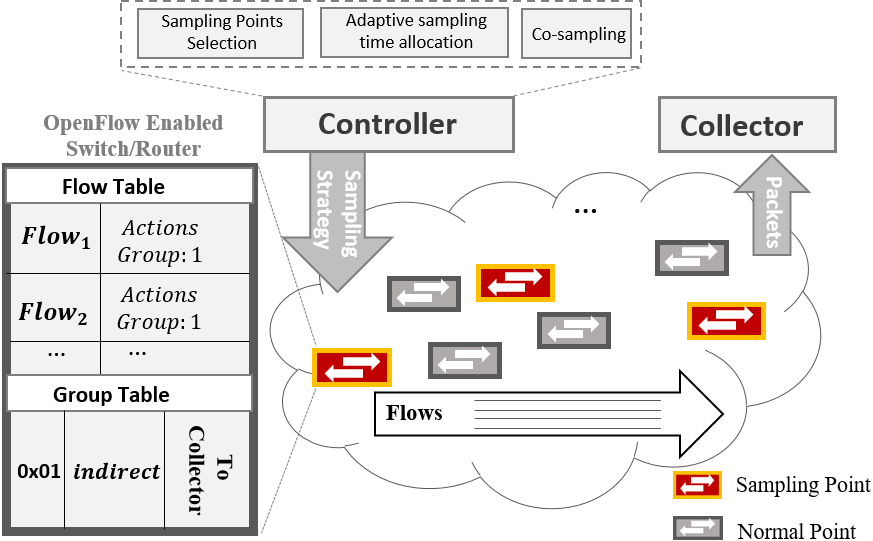
\includegraphics[width=8.5cm]{images/png_architecture.png}
\caption{The System Architecture Of AAA}
\label{aaa.png}
\end{figure}

\section{Related Work}
\begin{itemize}

\item A detailed introduction to the background: Why build an application-aware network - the contrast between traditional and SDN networks. 
\item Introducting the problems existing in building a large-scale application-aware network (a reasonable collection of traffic in a large-scale network environment is a basic problem in the field of traffic monitoring and traffic engineering). 
\item And including the solutions already on the basic problem, and the various problems that exist.
\item Introducting the Intermediary centrality algorithm.
\item Outline the algorithms and strategies we use.

\end{itemize}

\section{System Model and Design}

\subsection{Problem  Model}

We start with the four aspects of adaptability, agility, accuracy, efficiency, and synergy to abstract and model the problem. Build a AAA Co-Sampling Model. We abstract this problem with a new perspective, making the problem more intuitive and modeling the problem.

We believe that there is a cooperative relationship between the sampling between nodes. This relationship is multi-dimensional, which is reflected in the mutual constraint relationship between them, the coverage relationship of the current network, the static relationship in the topology, and so on.

Fig. 1 shows our intuitive abstraction of the problem. For a sampling period T, the stream set F in the entire network is like an area depicted by a red outline, and for R1..Rn, each node is covered with 0 or more streams, which is recorded as a set $F_i^c$, as shown in the flow information matrix, is a shaded area in gray in Fig. 1. The red dotted area is the newly arrived stream that may be covered by the period Ri corresponding to the period Ri. The overlapping area between the gray areas is the overlapping part of the flow covered between the nodes, $F_i^c \bigcap F_j^c$. The overlapping portion between the red dotted areas is the overlapping portion of the newly arrived flow covered between the nodes. Some nodes contain both gray and red areas; while some nodes only contain red or gray areas, which represents the value of each node in the period. The larger the area covered, the more streams the node covers. Therefore, the Flow-Level sampling problem can be intuitively converted to an area coverage maximization problem. That is, under the given collector processing power and other constraints, the sampling time allocation of each node is realized, so that the coverage area is maximized (the maximum number of stream coverage).

Under the definition of this problem, we propose a quantization model based on Slot partition time. Fig. 2 shows the way this model is used. First we divide the sampling period $T$ into $L$ equal length Slots; for each $Ri$, we need to determine its sampling Slot set $\widetilde S_i$. For any switch, the value it can generate in a Slot is expressed as $v_i$, which is visually represented as the number of streams sampled. For all nodes, the number and order of the Slots they are assigned to are calculated. The reason is that the number of Slots is positively correlated with the value generated by a node, and the more time is allocated to a node, The expected value of sampling to the stream is larger, and the order of the Slot of each node implicitly expresses the mutual constraint between the nodes: because the two nodes have overlapping flows, and when the coverage area is maximized, it should be removed. Multiple accumulations of overlapping areas between nodes in the same Slot. For the value $v_i$ produced by $R_i$, the quantization should take into account the expected number of known flows in a unit Slot time, and should also consider the number of new flows that may arrive within the period T, but For the unknown stream, even if we quantify the number of arrivals of a switch through the arrival distribution model of some flows, we cannot know the relationship between the unknown flows arriving between the nodes, and the paths and nodes of the unknown flow cannot be predicted. The relationship between the overlapping flows is so difficult to quantify the constraint relationship between the newly arrived flows to the nodes in the period $T$. However, for a node, its static Topology influence and short-term activity can be used to approximate its value in the period $T$. They represent one of the nodes in the week $T$ in the whole node. Influence, the greater the influence, the more likely it is to cover more flows. Moreover, these two attributes are private to the node, and there is no constraint relationship with other nodes. The number of known flows/the total number of streams covered by the nodes in the unit slot is the coverage of the current stream brought by the nodes in the unit time Slot, which we call the dynamic influence of the flow.

We give the following optimization model, Maximize Influence (formula), which is a transformation based on the traffic coverage problem: convert the number of coverage of the stream into coverage to quantify the node in unit $t$ Dynamic influence within; use Si and Hi to quantify the influence of nodes within $T$. Therefore, in $t$ unit time, the influence of a certain node should be considered in total and we use weighted way to get the comprehensive influence value of the node.
In the quantification of $D_i$, we assume that the arrival strength of the stream $f_i$ packet obeys the Poisson distribution with intensity $\lambda_i$.




\begin{equation}
\begin{split}
%\begin{gather}
\max \sum\limits_{i}^{n}{(\alpha \cdot \frac{\delta ({{v}_{i}},\left| \widetilde{{{S}_{i}}} \right|)}{\left| {{F}^{c}} \right|}+\frac{\left| \widetilde{{{S}_{i}}} \right|}{{T}/{t}\;}\cdot (\beta \cdot {{S}_{i}}+\gamma \cdot {{H}_{i}}))}  \\
-\frac{\alpha }{\left| {{F}^{c}} \right|}\cdot \sum\limits_{{{f}_{k}}\in {{F}^{c}}}{\sum\limits_{l=1}^{{T}/{t}\;}{\left( P\left\{ N_{p}^{k}\left( t \right)>0 \right\}\cdot \psi \left( {{f}_{k}},{{s}^{l}} \right) \right)}}
%\end{gather}
\end{split}
\end{equation}
subject to:
\begin{equation}
{v_i} = \sum\limits_{{f_k} \in {F^C}} {P\left\{ {N_p^k\left( t \right) > 0} \right\}}
\end{equation}
\begin{equation}
\delta \left( {{v_i},\left| {\widetilde {{S_i}}} \right|} \right) = \left\{ \begin{array}{l}
{v_i} \cdot \left| {\widetilde {{S_i}}} \right|,{\rm{    }}{v_i} \cdot \left| {\widetilde {{S_i}}} \right| < \left| {F_i^c} \right|\\
\left| {F_i^c} \right|{\rm{   }}\quad,\ {\rm{    ELSE}}
\end{array} \right.
\end{equation}
\begin{equation}
U = \left\{ {{R_i},{f_k} \in F_i^c \wedge {s^l} \in \widetilde {{S_i}}} \right\}
\end{equation}
\begin{equation}
\psi \left( {{f_k},{s^l}} \right) = \left\{ \begin{array}{l}
\left| U \right| - 1,{\rm{    }}\left| U \right| \ge 1\\
{\rm{   }}0\quad \quad \; \; ,\, \left| U \right| = 0
\end{array} \right.
\end{equation}

\begin{equation}
\alpha  + \beta  + \gamma  = 1
\end{equation}
\begin{equation}
\sum\nolimits_i^n {f(\widetilde {{S_i}}) \le } K,\quad f(\widetilde {{S_i}}) = \left\{ \begin{array}{l}
1,\ \ \left| {\widetilde {{S_i}}} \right| \ge 1\\
0,\ \ \left| {\widetilde {{S_i}}} \right| = 0
\end{array} \right.
\end{equation}
\begin{equation}
\sum\nolimits_i^n {{w_i} \cdot \varphi (\widetilde {{S_i}},{s^l}) \le C \cdot } t,{\rm{  }}\forall {{\rm{s}}^l} \wedge \varphi (\widetilde {{S_i}},{s^l}) = \left\{ \begin{array}{l}
0,{s^l} \notin \widetilde {{S_i}}\\
t,{s^l} \in \widetilde {{S_i}}
\end{array} \right.
\end{equation}
\begin{equation}
l \le {\raise0.7ex\hbox{$T$} \!\mathord{\left/
 {\vphantom {T t}}\right.\kern-\nulldelimiterspace}
\!\lower0.7ex\hbox{$t$}},\forall {s^l} \wedge t \le T
\end{equation}
\begin{equation}
K \le n,\forall {R_i}
\end{equation}
\begin{equation}
\left| {\widetilde {{S_i}}} \right| \le {\raise0.7ex\hbox{$T$} \!\mathord{\left/
 {\vphantom {T t}}\right.\kern-\nulldelimiterspace}
\!\lower0.7ex\hbox{$t$}},\forall i
\end{equation}

\begin{figure}[!!!!!!!!!!!!!!hhhhhhhhhht]
\centering
\subfigure[area coverage]
{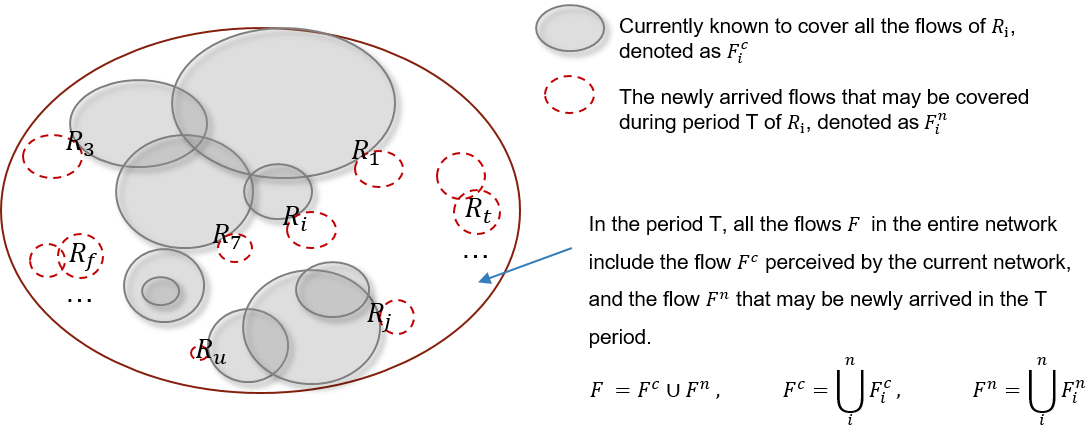
\includegraphics[width=8cm]{images/area_coverage.png}
\label{fig_1_area}
}

\subfigure[time slot allocation]
{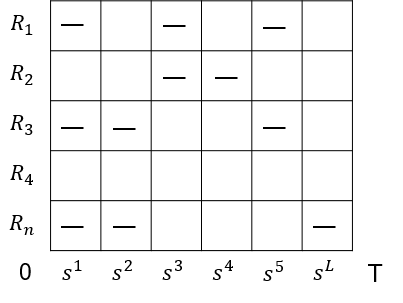
\includegraphics[width=8.5cm]{images/slot_num_order.png}
\label{fig_1_slot}
}
 
\caption{overview of model}
\label{fig_1_model}
\end{figure}


 

For the model of maximizing impact problems, the coverage of known traffic, the coverage of unknown new flows, the selection of nodes, the allocation of time slots, and the scheduling of Slot time series are fully considered. In the scheduling of time Slot, because the overlapping flows between nodes will cause conflicts under the same Slot, the overall coverage is reduced, so in order to get the optimal solution, the more overlapping the two nodes, if they are both When more than 0 Slots are allocated, the number of Slots they overlap should be as small as possible, which in turn solves another important sampling problem: how to reduce the problem of duplicate packets. Because each node contains the same stream, in order to optimize the results, it will be mutually exclusive on the Slot. Therefore, in the optimized solution, the sequence of $\widetilde S_i$ of each node can make the area covered by overlapping sampling in the whole cycle. Minimized, thus greatly reducing the repetition rate of the package while ensuring maximum sampling accuracy. Therefore, the nodes are cooperative, and through the constraint relationship between each other, the flow coverage relationship, the static topology relationship, the activity degree, etc., and finally maximize the number of sampled streams. (In the sampling process, when multiple nodes are sampled, a large number of duplicate packets are generated, because the stream may pass through any number of nodes, and the same packet will be collected at multiple nodes, which not only wastes valuable sampling resources, At the same time, the sampling accuracy is reduced. The repeated packets are reduced as much as possible, and the problem is avoided by the superposition relationship between the nodes, which not only improves the sampling accuracy, but also improves the efficiency of the upper application of the collector).

The model contains a number of sub-constrained sub-problems. We consider the complexity and feasibility while quantifying, and it is actually difficult to directly solve the solution to the problem. Therefore, we decompose the problem model into three sub-models: node selection, Slot number allocation, and Slot sequence arrangement. For each sub-problem, we model it independently and use an independent algorithm to solve the optimal solution or approximate optimal solution. In the end, the approximation of the problem can be effectively obtained.
This problem is not only a variant of multiple backpacks, but also adds enough constraints on the issue of multiple backpacks. Asking to solve this problem is an NP-hard problem. Therefore, we break it down into three parts to approximate the problem.

\begin{table}[h]
\centering
\caption{table}\label{tab:tab2}
\begin{tabular}{c|c}
\hline
Nonation & Explanation\\
\hline
\hline
M & the current flow information matrix \\
\hline
S & selected switches set \\
\hline
$sw_j$ & the $j$-th switch \\
\hline
$f_i$ & the $i$-th flow \\
\hline
$m_{ij}$ & the each value for $f_i$ and $sw_j$ in M,either 1 or 0 \\
\hline
$c_j$ & the betweenness centrality of $sw_j$  \\
\hline
$c_{max}$ & the max betweenness centrality of $sw_j$  \\
\hline
$I$ & the current number of flows  \\
\hline
$J$ & the current number of switches  \\
\hline
\hline
\end{tabular}
\end{table}

\subsection{Sampling Point Selection} 

According to the definition of model (1), select the K most influential nodes as sampling nodes and assign Slots.
In the optimization model (1), selecting the sampling node and assigning the number of Slots and determining the Slot order of each sampling node. The constraint between them is the overlapping problem of known flows between the nodes, so the three problems should be separated separately. First, the problem of overlapping of streams between nodes needs to be removed. We use the node influence power mode in model (1) to comprehensively quantify each node and select the top K influence maximization nodes through dynamic influence, static topological influence, and node historical influence. In the process of selecting the round (a total of K rounds), the high-impact nodes are used to privatize the overlapping flows to solve the overlapping problem of the flow. At this time, the dynamic influence force Di indicates the influence of the node based on the intermediate degree of the flow. Dik indicates the dynamic influence of node i when the kth node is selected during the Kth round selection. In the Kth round selection, if the i node has the greatest comprehensive influence, it will privatize all the flows it contains but Does not contain the stream contained in the nodes in the 1-k-1 round.
Formula (15) gives a quantitative formula for the comprehensive influence.

The principle of the algorithm will be stated next, with respect to the notations in Table I being used throughout the paper.

Firstly, initialize the matrix M=[$m_{ij}$] and the betweenness centrality $c_j$. Fig.\ref{png_sampling_point.png}-a shows a subnet topology, where there are 6 switch nodes and 6 flows. And we define: if $f_i$ passes through $sw_j$, the $m_{ij}$=1, otherwise $m_{ij}$=0. After initialization,as Fig.\ref{png_sampling_point.png}-b shows,we get a $I \ast J$ two-dimension matrix. Then calculate $c_j$ and $c_{max}$.

\begin{equation}
 c_{max} = \max\{ c_j \mid c_j=\sum_i{m_{ij}},i\in[1,I],j\in[1,J] \wedge  i,j\in Z\} 
\end{equation}
\begin{equation}
D_{i}^{k}={\left| {{F}_{i}}-\bigcup\nolimits_{c}^{k-1}{\widetilde{{{F}_{c}}}} \right|}/{\left| F-\bigcup\nolimits_{c}^{k-1}{\widetilde{{{F}_{c}}}} \right|}\;
\end{equation}
\begin{equation}
%{{H}_{i}}=\frac{T{{F}_{i}}}{TF}
{{H}_{i}}={T{{F}_{i}}}/{TF}\;
\end{equation}
\begin{equation}
%{{S}_{i}}=\frac{{{C}_{i}}}{\sum\nolimits_{i}^{n}{{{C}_{i}}}}
{{S}_{i}}={{{C}_{i}}}/{\sum\nolimits_{i}^{n}{{{C}_{i}}}}\;
\end{equation}
\begin{equation}
I_{i}^{k}=\alpha \cdot D_{i}^{k}+\beta \cdot {{S}_{i}}+\gamma \cdot {{H}_{i}}
\end{equation}

Senondly, elect the node with highest betweenness centrality as the sampling node and change $m_{ij}$ until each $m_{ij}$ = 0. As shown in Fig.\ref{png_sampling_point_in.png}, $c_{max}$ = $c_3$. Hence,the $sw_3$ is the first sampling node. Owing to $f_1$,$f_2$,$f_4$,$f_6$ pass through the $sw_3$, make $m_{ij}$ = 0($i$=1,2,4,6,$j \in [1,J]$). Then we can get a new marrix $M$ and calculate new $c_j$ and $c_{max}$ used for the next election. Repeating the above method, and electing the sampling node $sw_4$. Finally,we get $S$={$sw_3$,$sw_4$},when each $m_{ij}$=0.  

\begin{algorithm}[h]
\caption{Sampling Point Selection}
\begin{algorithmic}[1]
\REQUIRE ~~\\ The set of routers: $ R$ \\  The size of node will be selected: $K$ \\ The current flow information matrix: $M$
\STATE define $R^s=\{\}$  //  The Set of Selected Routers

\FOR{$k=1$; $k < K$; $k++$ }

\FOR{each $R_i \in R-R^s$}
\IF{$I_i^k > max$}
\STATE $max = I_i^k$
\STATE $SR = R_i$
\ENDIF
\ENDFOR
\STATE put $SR$ to $R^s$
\STATE mark $SR$ as $R_k$ in $R^s$
\ENDFOR

\RETURN $R^s$
\label{code:recentEnd}
\end{algorithmic}
\end{algorithm}



\begin{figure}[!hhhhhhhhhht]
\centering
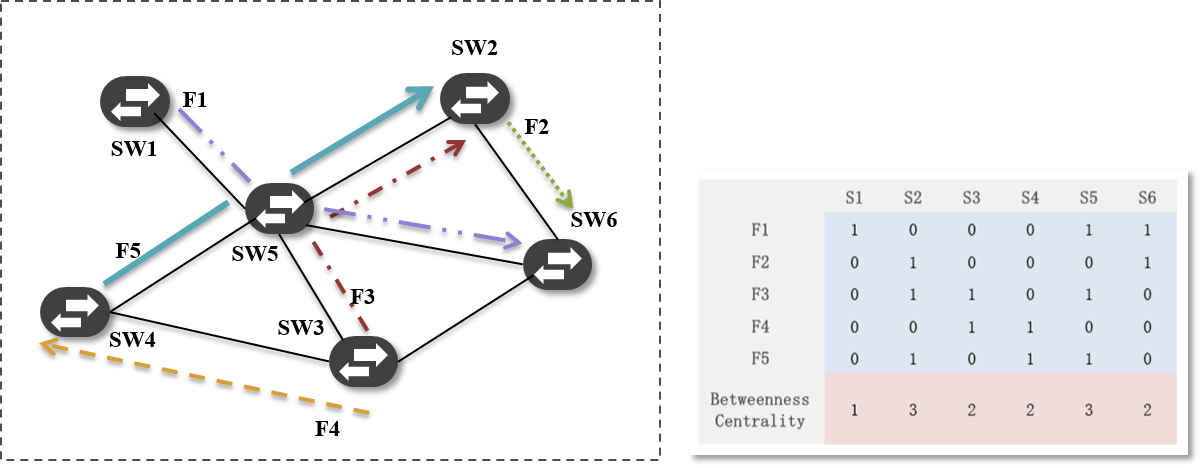
\includegraphics[width=8.5cm]{images/png_sampling_point.png}
\caption{Intermediary center based on the number of streams}
\label{png_sampling_point.png}
\end{figure}

\begin{figure}[!hhhhhhhhhht]
\centering
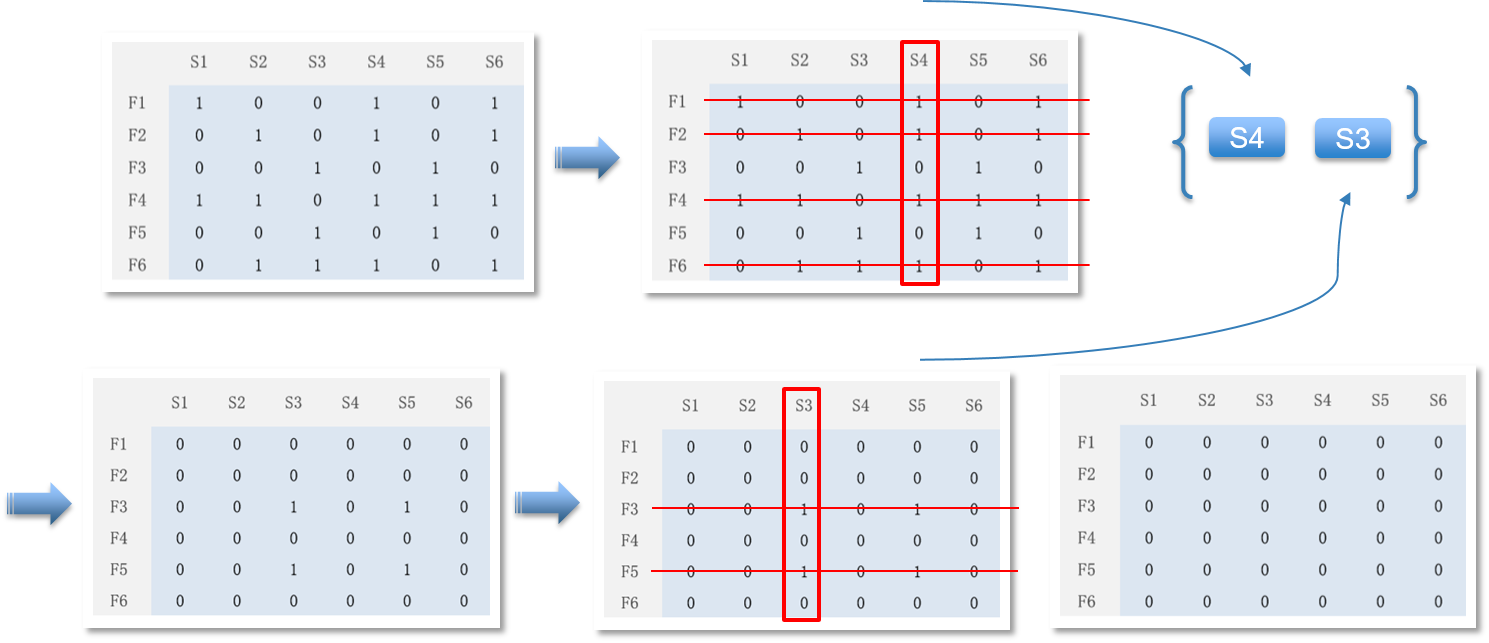
\includegraphics[width=8.5cm]{images/png_sampling_point_in.png}
\caption{Sampling Point Selection}
\label{png_sampling_point_in.png}
\end{figure}





\subsection{Allocation of Time Slot}


After the nodes are selected, each node needs to be assigned a number of slots. This is a typical multi-clip problem: there are a total of $K$ items to choose $(R^s_1-R^s_k)$, each type of item to be selected has $\frac{T}{t}$ ($\frac{T}{t}$ Slots can be selected), and each item is in one unit Slot t The benefit is $v(R_i, t_i)$ and the cost is $W(R_i, t_i)$. Therefore, we can use the algorithm for solving multiple backpacks to allocate the number of slots for each Ri. $v(R_i,t_i)$ is the part of Model(l)  in the model , take $ | \widetilde S |$ to 1. And $W(R_i, t_i)$ = the packet rate pkts/t of the unit t time Ri. When quantifying Di of $v(R_i, t_i)$, we assume in model (1) that the arrival rate of the packet of fi obeys the Poisson distribution. In the actual process, it is difficult to know the $\lambda $ intensity of the packet of a stream. We can pass fi The rate of the package to characterize.
When using multiple backpacks to solve this problem, there may be a phenomenon of hunger distribution: some low-impact nodes are assigned to 0 slots. This phenomenon is not avoided. We assign a Slot to each node from the high-impact to low-impact nodes (Rs1-Rsk) in advance (in the case where the cost does not exceed the total constraint), and then use multiple backpacks to solve You can try to avoid hunger.

When solving multiple backpacks, in addition to the problem of hunger, the solution efficiency is the complexity of $O(n^2)$. When $T$ is too large or t is too small and C is large, it is unacceptable to solve the optimal solution time. We give a simple and efficient strategy. Algorithm 2 shows this approach.

\begin{algorithm}[h]
\caption{Allocation of Time Slot Based on XXX}
\begin{algorithmic}[1]
\REQUIRE  $K$~,$L$~,$C$~, weight $W=\{w_1,w_2...,w_k\}$~,value $V=\{v_1,v_2...,v_k\}$
\WHILE{$C > 0$}
\STATE $Cas = 1$
\FOR{$k=1$; $k < K$; $k++$}
\IF{$C >= w_i*Cas$}
\STATE $count[i]+= Cas$
\STATE $C = C - w_i * Cas$
\ENDIF
\ENDFOR
\ENDWHILE
\RETURN reverse~iteration,output~$N=\{n_{1},n_{2}...,n_{k}\}$
\label{code:recentEnd}
\end{algorithmic}
\end{algorithm}


\subsection{Order of Time Slot}

Determining time series for each node, in Model(1), reflects the effects of overlapping relationships between nodes, such as the accuracy of the sampling of the system and the repetition rate of the sample packets. In the second chapter, we use the high-impact privatization of overlapping flows to approximate the effect of the precision caused by overlapping flows between nodes. Therefore, in this section, we reduce the repetition rate of the packet by optimizing the sampling sequence of each node Slot.

This optimization problem can be defined by the following formula(16). Where $ \left| \widetilde{{{S}_{i}}}\bigcap \widetilde{{{S}_{j}}} \right| $ represents the number of overlaps of the time slots of the two nodes, and $\left| \widetilde{{{F}_{i}}}\bigcap \widetilde{{{F}_{j}}} \right|$ represents the number of overlapping flows between the two nodes of ij. Therefore, this formula embodies the overlap area of the flow in the entire sampling system.

\begin{equation}
\min \sum{(\left| \widetilde{{{S}_{i}}}\bigcap \widetilde{{{S}_{j}}} \right|}\cdot \left| \widetilde{{{F}_{i}}}\bigcap \widetilde{{{F}_{j}}} \right|),\forall i,j\wedge i\ne j
\end{equation}

From the definition of the problem, the search backtracking method can be used to solve the optimal solution, but it is a problem that cannot be solved in a polynomial time. Therefore, we consider a simple greedy algorithm to solve the approximate optimal solution of the problem.
 
\begin{algorithm}[h]
\caption{Order of Time Slot Based on Greedy}
\begin{algorithmic}[1]
\REQUIRE  $M$ ~, $S$ ~, $c_j$
\WHILE{$CNT[i] > 0,\exists i \wedge i = 1,2...,k$}
\FOR{$i=1$; $i <= K$; $i++$}
\IF{$CNT[i] > 0$}
\STATE $Min = Max$ $Integer$
\FOR{$l=1$; $l < \frac{T}{t}$; $l++$}
\IF{$M^{slot}[i][l] = 0$}
\STATE $temp = \sum^{K}_{j=1 \wedge j != i}(\left| \widetilde{{{F}_{i}}}\bigcap \widetilde{{{F}_{j}}} \right| \cdot M^{slot}[j][l]) + H[j] $
\IF{$temp < Min$}
\STATE $Min = temp$; $Sp = l$ 
\ENDIF
\ENDIF
\ENDFOR
\STATE$M^{slot}[i][Sp] = 1$; $ CNT[i]--$; $H[Sp] = Min$
\ENDIF
\ENDFOR
\ENDWHILE

\RETURN $M^{slot}$
\label{code:recentEnd}
\end{algorithmic}
\end{algorithm}

\begin{figure}[!hhhhhhhhhht]
\centering
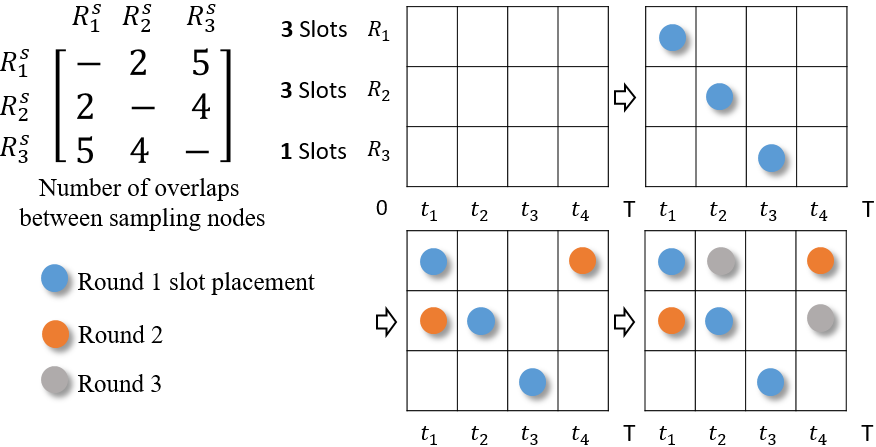
\includegraphics[width=8cm]{images/greedy_for_order_slot.png}
\caption{comparison of sampling flow number at different slot}
\label{aaa.png}
\end{figure}

\section{Experiments and results}
In order to verify the effectiveness and performance of our algorithm, we have built a laboratory bed based on floodlight controller and openvswitch + mininet. The whole experimental bed contains 12 Dell XPS hosts, 20 core CPU, and Ubuntu 16.06.2 LTS. One runs a floodlight controller that fuses our algorithm, the other runs a data collector, and the remaining 10 deploy a network topology with 110 switch nodes and 50 host nodes. The experimental traffic dataset comes from the open project "the WIDE Project". We selected data from 14:00-14:15 in August 6, 2018. After cleaning and screening, we collate 5000 data streams for experiments. In the experiment, the number of data streams changed from 1000 to 5000..
We implement four algorithms: Random-K, top-K based on the extended median centrality, top-K based on the standard median centrality, our algorithm XXX. Based on the above four algorithms, we have made a comparative experiment in three measurement mechanisms: sampling accuracy, packet repetition rate and the number of rat streams collected.
Fig.x shows the comparison of sampling accuracy in different algorithms. Our algorithm is 7\% higher than Top-k and over 20\% than the other two algorithms. From Fig.x, we can see that different algorithms do almost the same amount of elephant flow collection. In fact, our algorithm only takes more part of the rat flow than other algorithms. And Fig.x shows that our algorithm is effective in reducing duplication and reducing it by more than 30\%.

%\begin{figure}[!hhhhhhhhhht]
%\centering
%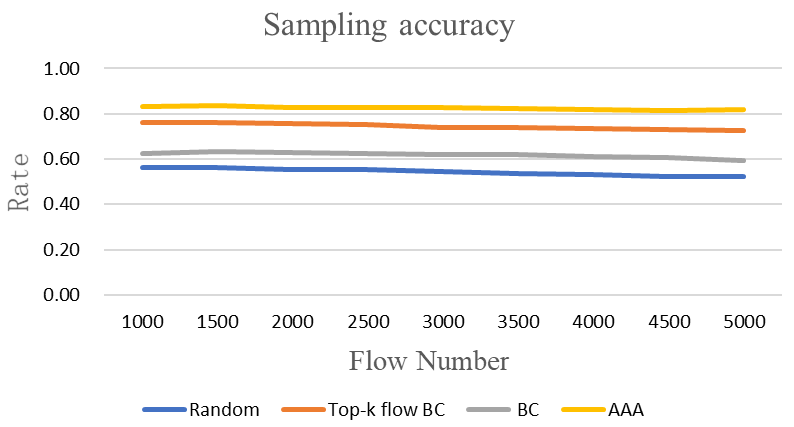
\includegraphics[width=8cm]{images/cmp_sam_accu.png}
%\caption{accuracy comparison with respect to different algorithms}
%\label{aaa.png}
%\end{figure}

\begin{figure}[!!!!!!!!!!!!!!hhhhhhhhhht]
\centering
\subfigure[ comparison of sampling accuracy]
{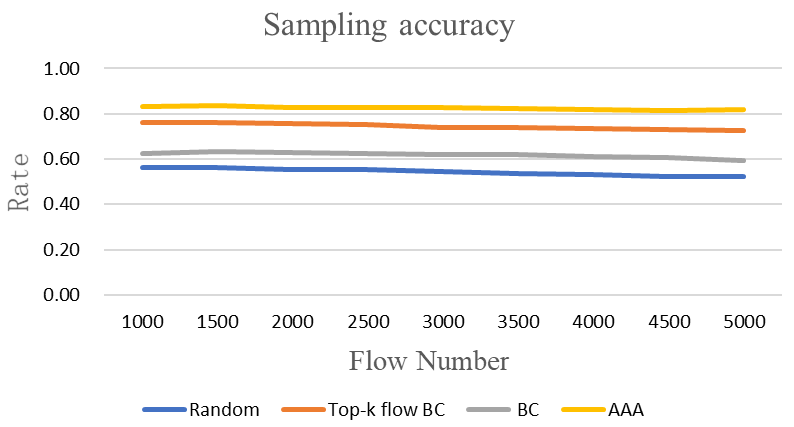
\includegraphics[width=4.1cm]{images/cmp_sam_accu.png}
\label{fig_x_accu}
}
\subfigure[comparison of repetition rate]
{\includegraphics[width=4.1cm]{images//cmp_rep_rate.png}
\label{fig_x_rep}
}
\caption{comparison with respect to different algorithms}
\label{fig_x_cmp}
\end{figure}

\begin{figure}[!hhhhhhhhhht]
\centering
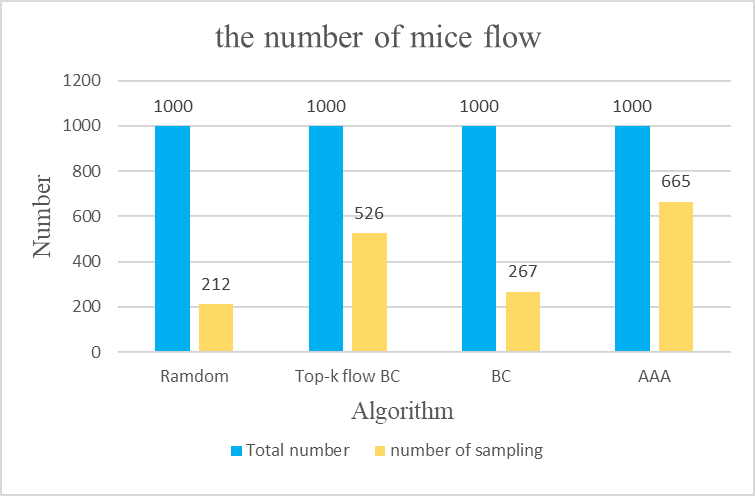
\includegraphics[width=8cm]{images/cmp_mice_flownum.png}
\caption{comparison of different algorithms in number of mice flow}
\label{aaa.png}
\end{figure}

\begin{figure}[!hhhhhhhhhht]
\centering
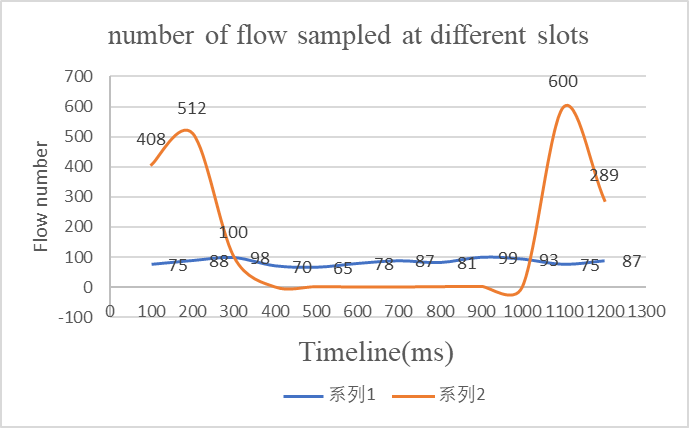
\includegraphics[width=8cm]{images/num_slot.png}
\caption{comparison of sampling flow number at different slot}
\label{aaa.png}
\end{figure}

%\begin{figure}[!hhhhhhhhhht]
%\centering
%\includegraphics[width=8cm]{images/cmp_rep_rate.png}
%\caption{repetition rate comparison with respect to different algorithms }
%\label{aaa.png}
%\end{figure}


 





 


\section{Conclusion}
\begin{itemize}
\item Lab environment
\item Sampling accuracy comparison
\item Sampling repetition rate comparison
\item Greedy centrality algorithm experimental results
 
\item Deduplication rate algorithm comparison

\item Experimental comparison of adaptive co-sampling algorithm
\end{itemize}



%\section{Conclusion}

%\begin{itemize}
%\item[-] Case 1: $ \frac{1}{SW_{num}} < S_{rate} \Leftrightarrow Confliction $   \\
%\item[-] Case 2: $ \frac{1}{SW_{num}} >= S_{rate} \Leftrightarrow no Confliction $ 


 





% trigger a \newpage just before the given reference
% number - used to balance the columns on the last page
% adjust value as needed - may need to be readjusted if
% the document is modified later
%\IEEEtriggeratref{8}
% The "triggered" command can be changed if desired:
%\IEEEtriggercmd{\enlargethispage{-5in}}

% references section

% can use a bibliography generated by BibTeX as a .bbl file
% BibTeX documentation can be easily obtained at:
% http://mirror.ctan.org/biblio/bibtex/contrib/doc/
% The IEEEtran BibTeX style support page is at:
% http://www.michaelshell.org/tex/ieeetran/bibtex/
%\bibliographystyle{IEEEtran}
% argument is your BibTeX string definitions and bibliography database(s)
%\bibliography{IEEEabrv,../bib/paper}
%
% <OR> manually copy in the resultant .bbl file
% set second argument of \begin to the number of references
% (used to reserve space for the reference number labels box)
\begin{thebibliography}{1}

\bibitem{1}
S.~Yoon, T.~Ha, S.~Kim and H.~Lim,\hskip 1em plus 0.5em minus 0.4em
Scalable Traffic Sampling using Centrality Measure on Software-Defined Networks, in \emph{IEEE Communications Magazine}, pp.43-49, July 2017.

\bibitem{1}
M.~Malboubi, L.~Wang, C.N.~Chuah, P.~Sharma,\hskip 1em plus 0.5em minus 0.4em
Intelligent SDN based Traffic (de)Aggregation and Measurement Paradigm (iSTAMP), in \emph{IEEE INFOCOM}, Apr 2014.

\bibitem{1}
L.~Tong and W.~Gao,\hskip 1em plus 0.5em minus 0.4em
Application-Aware Traffic Scheduling for Workload Offloading in Mobile Clouds, in \emph{IEEE INFOCOM}, pp.1-9, Apr 2016.

\bibitem{1}
J.~Jiang, S.~Ma, B.~Li and B.~Li,\hskip 1em plus 0.5em minus 0.4em
Symbiosis: Network-Aware Task Scheduling in Data-Parallel Frameworks, in \emph{IEEE INFOCOM}, pp.10-14, Apr 2016.

\bibitem{1}
P.~Bakopoulos, K.~Christodoulopoulos, G.~Landi et al,\hskip 1em plus 0.5em minus 0.4em
NEPHELE: An End-to-End Scalable and Dynamically Reconfgurable Optical Architecture for Application-Aware SDN Cloud Data Centers, in \emph{IEEE Communitions Magazine}, pp.178-188, Feb 2018.

\bibitem{2}
J.~Xu, J.Y.~Wang, Q.~Qi, H.F.~Sun and B.~He,\hskip 1em plus 0.5em minus 0.4em
IARA: An Intelligent Application-aware VNF for Network Resource Allocation with Deep Learning, in \emph{IEEE SECON}, pp.1-3, June 2018.

\bibitem{2}
J.~Suh, T.T.~Kwon, C.~Dixon, W.~Felter and J.~Carter,\hskip 1em plus 0.5em minus 0.4em
OpenSample: A Low-latency, Sampling-based Measurement Platform for Commodity SDN, in \emph{IEEE ICDCS}, pp.228-237, July 2014.

\bibitem{2}
Z.~Su, T.~Wang, Y.~Xia and M.~Hamdi,\hskip 1em plus 0.5em minus 0.4em
CeMon: A Cost-effective Flow Monitoring System in Software Defined Networks, in \emph{Computer Networks}, pp.101-115, Dec 2015.

\bibitem{3}
N.F.~Huang, C.C.~Li, C.H.~Li, C.C.~Chen,C.H.~C and I.H.~Hsu,\hskip 1em plus 0.5em minus 0.4em
Application Identification System or SDN QoS based on Machine Learning and DNS Responses, in \emph{APNOMS}, pp.407-410, Sept 2017.

\bibitem{3}
S.~Jeong, D.~Lee, J.~Hyun, J.~Li, and J.W.~Hong,\hskip 1em plus 0.5em minus 0.4em
Application-aware Traffic Engineering in Software-Defined Network, in \emph{APNOMS}, pp.315-318, Sept 2017.

\bibitem{3}
G.~Cheng and Y.~Tang,\hskip 1em plus 0.5em minus 0.4em
eOpenFlow: Software Defined Sampling via a Highly Adoptable OpenFlow Extension, in \emph{IEEE ICC}, pp.1-6, May 2017.


\bibitem{3}
S.~Zhao and D.~Medhi,\hskip 1em plus 0.5em minus 0.4em
Application Performance Optimization Using Application-Aware Networking, in \emph{IEEE NOMS},pp.1-6, Apr 2018.

\bibitem{4}
M.~Malboubi, S.M.~Peng, P.~Sharma and C.N.~Chuah,\hskip 1em plus 0.5em minus 0.4em
A Learning-based Measurement Framework for Traffic Matrix Inference in Software Defined Networks, in \emph{Computers \& Electrical Engineering}, Dec 2017.

\bibitem{4}
K.~Bilal, S.U.~Khan, L.~Zhang et al,\hskip 1em plus 0.5em minus 0.4em
Quantitative comparisons of the state-of-the-art data center architectures, in \emph{Concurrency \& Computation Practice \& Experience}, Dec 2017.

\end{thebibliography}




% that's all folks
\end{document}


